
%%--------------------------------------------------
%% CPO: Multiple Choice Questions
%%--------------------------------------------------


%% Chapter 21: Sound
%%--------------------------------------------------


%% Learning Objectives
%%--------------------------------------------------

%% Explain how pitch, loudness, and speed are related to waves. 
%% Explain the Doppler effect. 
%% Describe how sound is created and recorded.
%% Explain how sound is made and know the factors that affect the speed of sound. 
%% Know that the speed of sound changes in different materials. 
%% Explain the importance of the wavelength of sound.
%% Describe sound interactions. 
%% Compare the superposition principle and Fourier's theorem. 
%% Describe how the meaning of sound is related to frequency and time. 
%% Explain how we hear sound. 
%% Describe the musical scale, consonance, dissonance, and beats in terms of sound waves. 
%% Describe the role of harmonics in how instruments sound.


%% CPO Multiple Choice Questions
%%--------------------------------------------------
\element{cpo-mc}{
\begin{question}{cpo-ch21-q01}
    The musical term ``pitch'' is most directly proportional to:
    \begin{multicols}{2}
    \begin{choices}
        \wrongchoice{amplitude}
        \wrongchoice{volume}
        \wrongchoice{wavelength}
      \correctchoice{frequency}
    \end{choices}
    \end{multicols}
\end{question}
}

\element{cpo-mc}{
\begin{question}{cpo-ch21-q02}
    The loudness of sound is measured in units called:
    \begin{multicols}{2}
    \begin{choices}
        \wrongchoice{newton (\si{\newton})}
        \wrongchoice{pascal (\si{\pascal})}
        \wrongchoice{hertz (\si{\hertz})}
      \correctchoice{decibel (\si{\decibel})}
    \end{choices}
    \end{multicols}
\end{question}
}

\element{cpo-mc}{
\begin{question}{cpo-ch21-q03}
    Ordinary conversation, measured in decibel units,
        would be most nearly:
    \begin{multicols}{2}
    \begin{choices}
        \wrongchoice{\SI{15}{\decibel}}
      \correctchoice{\SI{65}{\decibel}}
        \wrongchoice{\SI{100}{\decibel}}
        \wrongchoice{\SI{125}{\decibel}}
    \end{choices}
    \end{multicols}
\end{question}
}

\element{cpo-mc}{
\begin{question}{cpo-ch21-q04}
    The term applied to objects that travel at speeds exceeding the normal speed of sound in air is:
    \begin{multicols}{2}
    \begin{choices}
        \wrongchoice{subsonic}
      \correctchoice{supersonic}
        \wrongchoice{sonogram}
        \wrongchoice{reverberation}
    \end{choices}
    \end{multicols}
\end{question}
}

\element{cpo-mc}{
\begin{question}{cpo-ch21-q05}
    As the decibel level increases from \SI{20}{\decibel} to \SI{40}{\decibel},
        the loudness of the sound is described as:
    \begin{multicols}{2}
    \begin{choices}
        \wrongchoice{10 times louder}
      \correctchoice{2 times louder}
        \wrongchoice{10 times quieter}
        \wrongchoice{2 times quieter}
    \end{choices}
    \end{multicols}
\end{question}
}

\element{cpo-mc}{
\begin{question}{cpo-ch21-q06}
    Due to the Doppler effect,
        the pitch of the siren of a fire truck moving away from you:
    \begin{choices}
      \correctchoice{decreases}
        \wrongchoice{increases}
        \wrongchoice{increases then decreases}
        \wrongchoice{does not change}
    \end{choices}
\end{question}
}

\element{cpo-mc}{
\begin{question}{cpo-ch21-q07}
    The four diagrams below represent the amplitude of sounds produced versus time.
    Which diagram represents a complex sound?
    \begin{multicols}{2}
    \begin{choices}
        \AMCboxDimensions{down=-1.0cm}
        \correctchoice{
            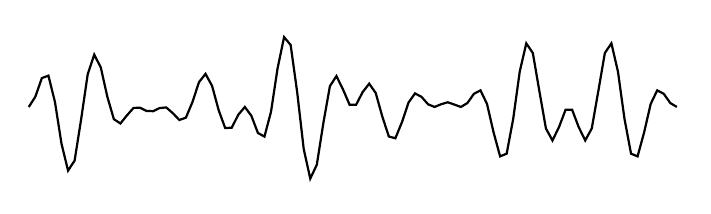
\begin{tikzpicture}[x=0.018\columnwidth]
                \draw[draw=white] (0,-1.0) to (38,1.0);
                \draw[domain=0:12*pi,samples=100,thick] plot (\x, {cos(0.2*\x r)*sin(2*\x r)*sin(0.5*\x r)});
            \end{tikzpicture}
        }
        \wrongchoice{
            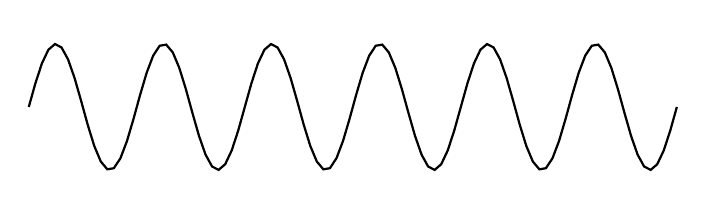
\begin{tikzpicture}[x=0.018\columnwidth]
                \draw[draw=white] (0,-1.0) to (38,1.0);
                \draw[domain=0:12*pi,samples=100,thick] plot (\x, {0.8*sin(\x r)});
            \end{tikzpicture}
        }
        \wrongchoice{
            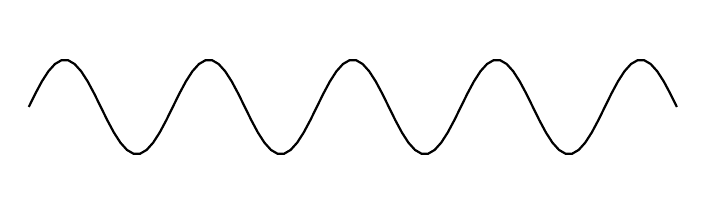
\begin{tikzpicture}[x=0.018\columnwidth]
                \draw[draw=white] (0,-1.0) to (38,1.0);
                \draw[domain=0:12*pi,samples=100,thick] plot (\x, {0.6*sin(0.75*\x r)});
            \end{tikzpicture}
        }
        \wrongchoice{
            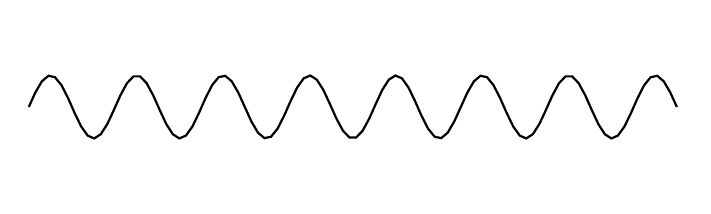
\begin{tikzpicture}[x=0.018\columnwidth]
                \draw[draw=white] (0,-1.0) to (38,1.0);
                \draw[domain=0:12*pi,samples=100,thick] plot (\x, {0.4*sin(1.25*\x r)});
            \end{tikzpicture}
        }
    \end{choices}
    \end{multicols}
\end{question}
}

\element{cpo-mc}{
\begin{question}{cpo-ch21-q08}
    Sound will travel:
    \begin{choices}
        \wrongchoice{faster in air than in any material.}
        \wrongchoice{fastest in outer space.}
      \correctchoice{faster in steel than in air.}
        \wrongchoice{faster in cold air than warm air.}
    \end{choices}
\end{question}
}

%% REF: http://www.texample.net/tikz/examples/brillouin-function/
%% REF: http://mariobon.com/Glossario/Loudness_ISO_226_2003b.pdf
%% REF: http://www.dsprelated.com/showcode/174.php
%% REF: http://zainea.com/equalloudnesslevel.pdf

\element{cpo-mc}{
\begin{question}{cpo-ch21-q09}
    According to the \emph{Equal Loudness Curves} graph,
        as the frequency of a sound decreases from \SI{2 000}{\hertz} to \SI{50}{\hertz},
        the human ear's sensitivity to the loudness of that sound:
    %% Define Equal Loudness Functions
    \directlua{dofile('./qbank/cpo/equalLoudness.lua')}
    \begin{center}
    \begin{tikzpicture}
        \begin{semilogxaxis}[
            axis y line=left,
            axis x line=bottom,
            axis line style={->},
            title={Equal Loudness Curves},
            ylabel={Sound Pressure Level},
            y unit=\si{\decibel},
            ymin=0,ymax=125,
            xlabel={Frequency},
            x unit=\si{\hertz},
            xmin=2e1,xmax=2e4,
            no marks,
        ]
        \foreach \k in {20,30,...,90}{
            \directlua{printEqualLoudnessCurve(\k)}
        }
        \end{semilogxaxis}
    \end{tikzpicture}
    \end{center}
    \begin{choices}
        \wrongchoice{increases.}
      \correctchoice{decreases.}
        \wrongchoice{is equal.}
        \wrongchoice{depends on the source.}
    \end{choices}
\end{question}
}

\element{cpo-mc}{
\begin{question}{cpo-ch21-q10}
    You yell across the bottom of a wide canyon and hear your echo \SI{3}{\second} later.
    The approximate width of the canyon producing the echo is:
    \begin{multicols}{2}
    \begin{choices}
        \wrongchoice{\SI{1 000}{\meter}}
      \correctchoice{\SI{500}{\meter}}
        \wrongchoice{\SI{300}{\meter}}
        \wrongchoice{\SI{100}{\meter}}
    \end{choices}
    \end{multicols}
\end{question}
}

\element{cpo-mc}{
\begin{question}{cpo-ch21-q11}
    Ultrasound is useful for all of the following \emph{except}:
    \begin{choices}
        \wrongchoice{examining a beating heart.}
      \correctchoice{placing mp3 files on a CD.}
        \wrongchoice{detecting structural damage in materials.}
        \wrongchoice{determining the gender of an unborn child.}
    \end{choices}
\end{question}
}

\element{cpo-mc}{
\begin{question}{cpo-ch21-q12}
    A large explosion generally can be ``felt'' some distance away and is the source of a low frequency sound because it causes a variation in the:
    \begin{choices}
        \wrongchoice{air temperature.}
      \correctchoice{air pressure.}
        \wrongchoice{mass of air molecules.}
        \wrongchoice{weight of air molecules.}
    \end{choices}
\end{question}
}

\element{cpo-mc}{
\begin{question}{cpo-ch21-q13}
    Sound shows wave characteristics for all of the following reasons \emph{except}:
    \begin{choices}
      \correctchoice{the mass of sound increases as its frequency increases.}
        \wrongchoice{sound may be reflected and refracted.}
        \wrongchoice{the speed of sound is the product of frequency and wavelength.}
        \wrongchoice{sound shows evidence of diffraction and interference.}
    \end{choices}
\end{question}
}

\element{cpo-mc}{
\begin{question}{cpo-ch21-q14}
    The speed of sound in air at normal temperatures is about:
    \begin{multicols}{2}
    \begin{choices}
        \wrongchoice{\SI{34}{\meter\per\second}}
      \correctchoice{\SI{340}{\meter\per\second}}
        \wrongchoice{\SI{3 400}{\meter\per\second}}
        \wrongchoice{\SI{34 000}{\meter\per\second}}
    \end{choices}
    \end{multicols}
\end{question}
}

\element{cpo-mc}{
\begin{question}{cpo-ch21-q15}
    The speed of sound is affected by all of the following \emph{except}:
    \begin{choices}
      \correctchoice{decibel level}
        \wrongchoice{air pressure}
        \wrongchoice{temperature}
        \wrongchoice{weight and size of the molecules it travels through}
    \end{choices}
\end{question}
}

\element{cpo-mc}{
\begin{question}{cpo-ch21-q16}
    Which of the following statements about reverberations is \emph{incorrect}?
    \begin{choices}
        \wrongchoice{Reverberations may create dead spots in a large room.}
        \wrongchoice{Reverberations may cause loud spots in a large room.}
      \correctchoice{Reverberations are caused by absorption of sound by concert hall walls and ceilings.}
        \wrongchoice{The source of reverberation is multiple echoes from concert hall walls and ceilings.}
    \end{choices}
\end{question}
}

\element{cpo-mc}{
\begin{question}{cpo-ch21-q17}
    The oscillation of air pressure can result in:
    \begin{choices}
        \wrongchoice{transverse waves}
        \wrongchoice{light waves}
      \correctchoice{longitudinal waves}
        \wrongchoice{circular waves}
    \end{choices}
\end{question}
}

\element{cpo-mc}{
\begin{question}{cpo-ch21-q18}
    Large horns such as tubas produce sounds with long wavelength while flutes produce sounds with short wavelength because:
    \begin{choices}
        \wrongchoice{the frequency of sound produced is directly proportional to the size of the instrument.}
      \correctchoice{the wavelength of sound produced is directly proportional to the size of the instrument.}
        \wrongchoice{the wavelength of sound produced is directly proportional to the frequency.}
        \wrongchoice{the pitch of the sound produced is directly proportional to the wavelength.}
    \end{choices}
\end{question}
}

\element{cpo-mc}{
\begin{question}{cpo-ch21-q19}
    Which of the following has the shortest wavelength?
    \begin{choices}
        \wrongchoice{A rumble of thunder at \SI{20}{\hertz}.}
        \wrongchoice{An average male singer at \SI{500}{\hertz}.}
        \wrongchoice{The highest note on a piano at \SI{5 000}{\hertz}.}
      \correctchoice{The whine of a jet turbine at \SI{10 000}{\hertz}.}
    \end{choices}
\end{question}
}

\element{cpo-mc}{
\begin{question}{cpo-ch21-q20}
    The marching band is practicing behind the school.
    In front of the school,
        students are able to hear the band because the sound waves are:
    \begin{choices}
        \wrongchoice{absorbed by the building and trees}
      \correctchoice{diffracted over and around the school}
        \wrongchoice{refracted by the school building}
        \wrongchoice{enhanced by destructive interference}
    \end{choices}
\end{question}
}

\element{cpo-mc}{
\begin{question}{cpo-ch21-q21}
    On the Fourth of July,
        you can see large fireworks displays before you hear them because the speed of light exceeds the speed of sound by a factor of:
    \begin{multicols}{2}
    \begin{choices}
        \wrongchoice{\num{10}}
        \wrongchoice{\num{1 000}}
        \wrongchoice{\num{100 000}}
      \correctchoice{\num{1 000 000}}
    \end{choices}
    \end{multicols}
\end{question}
}

\element{cpo-mc}{
\begin{questionmult}{ch21-Q22}
    The perception of sound starts with the:
    \begin{choices}
        \wrongchoice{stimulation of the fluid in the cochlea}
        \wrongchoice{response of short hairs of the ear canal}
        \wrongchoice{movement of three delicate bones of the inner ear}
      \correctchoice{vibration of the eardrum}
    \end{choices}
\end{questionmult}
}

\element{cpo-mc}{
\begin{question}{cpo-ch21-q23}
    The term for a regular time pattern in sound is:
    \begin{multicols}{2}
    \begin{choices}
      \correctchoice{rhythm}
        \wrongchoice{pitch}
        \wrongchoice{scale}
        \wrongchoice{harmony}
    \end{choices}
    \end{multicols}
\end{question}
}

\element{cpo-mc}{
\begin{question}{cpo-ch21-q24}
    The musical effect based upon the relationship between frequencies can be called:
    \begin{multicols}{2}
    \begin{choices}
        \wrongchoice{pitch}
      \correctchoice{harmony}
        \wrongchoice{beats}
        \wrongchoice{rhythm}
    \end{choices}
    \end{multicols}
\end{question}
}

\element{cpo-mc}{
\begin{question}{cpo-ch21-q25}
    Musicians may tune their instruments to match a certain frequency by adjusting the frequency they play to eliminate:
    \begin{multicols}{2}
    \begin{choices}
        \wrongchoice{scales}
        \wrongchoice{rhythm}
        \wrongchoice{pitch}
      \correctchoice{beats}
    \end{choices}
    \end{multicols}
\end{question}
}

\element{cpo-mc}{
\begin{question}{cpo-ch21-q26}
    The property of sound that most helps you to identify one person's voice from another is:
    \begin{multicols}{2}
    \begin{choices}
        \wrongchoice{decibels}
        \wrongchoice{beats}
      \correctchoice{harmonics}
        \wrongchoice{scales}
    \end{choices}
    \end{multicols}
\end{question}
}

\element{cpo-mc}{
\begin{question}{cpo-ch21-q27}
    A piano and a guitar playing the same ``C'' note sound different because pianos:
    \begin{choices}
        \wrongchoice{produce sound with more decibels}
      \correctchoice{and guitars produce different combinations of frequencies}
        \wrongchoice{produce pure frequencies but guitars do not}
        \wrongchoice{have more ``strings'' (wires) to vibrate than guitars}
    \end{choices}
\end{question}
}

\element{cpo-mc}{
\begin{question}{cpo-ch21-q28}
    A special graph of sound displaying the frequency versus time while indicating how loud the sound is at various frequencies is called a(n):
    \begin{choices}
      \correctchoice{sonogram}
        \wrongchoice{equal loudness curve}
        \wrongchoice{ultrasound}
        \wrongchoice{spectrum}
    \end{choices}
\end{question}
}

\element{cpo-mc}{
\begin{question}{cpo-ch21-q29}
    A combination of frequencies which sounds bad or is unsettling is called:
    \begin{multicols}{2}
    \begin{choices}
      \correctchoice{dissonance}
        \wrongchoice{consonance}
        \wrongchoice{harmony}
        \wrongchoice{pitch}
    \end{choices}
    \end{multicols}
\end{question}
}

\element{cpo-mc}{
\begin{question}{cpo-ch21-q30}
    While a young child is able to hear frequencies of sound up to \SI{20 000}{\hertz},
        the highest frequencies an average adult is able to hear is:
    \begin{multicols}{2}
    \begin{choices}
        \wrongchoice{\SI{2 000}{\hertz}}
        \wrongchoice{\SI{5 000}{\hertz}}
      \correctchoice{\SI{15 000}{\hertz}}
        \wrongchoice{\SI{22 000}{\hertz}}
    \end{choices}
    \end{multicols}
\end{question}
}

\element{cpo-mc}{
\begin{question}{cpo-ch21-q31}
    A guitar player controls the notes produced by placing her fingers at specific positions on the strings.
    The notes are produced as a result of:
    \begin{multicols}{2}
    \begin{choices}
        \wrongchoice{diffraction}
        \wrongchoice{polarization}
      \correctchoice{resonance}
        \wrongchoice{refraction}
    \end{choices}
    \end{multicols}
\end{question}
}

\element{cpo-mc}{
\begin{question}{cpo-ch21-q32}
    Loud noises damage the ear because:
    \begin{choices}
        \wrongchoice{they can block the ear canal}
        \wrongchoice{they are transmitted to the ear faster in the atmosphere than quiet noises}
      \correctchoice{they can cause tiny hairs in the cochlea to break}
        \wrongchoice{their frequency exceeds \SI{20 000}{\hertz}}
    \end{choices}
\end{question}
}

\endinput


